\documentclass[12pt, a4paper]{article}
\usepackage[utf8]{inputenc}
\usepackage{graphicx}
\usepackage{listings}
\usepackage{xcolor}
\usepackage{geometry}
\usepackage{float}
\usepackage{hyperref}
\usepackage{booktabs}
\usepackage{tikz}
\usepackage{amsmath}
\usepackage{caption}
\usepackage{setspace}
\usetikzlibrary{shapes.geometric, arrows, positioning}

% Page Layout - wider margins for a cleaner look
\geometry{margin=1in}
\setlength{\parskip}{1.2em}
\setlength{\parindent}{0pt}
\onehalfspacing

% Colors for code listings
\definecolor{codegreen}{rgb}{0,0.6,0}
\definecolor{codegray}{rgb}{0.5,0.5,0.5}
\definecolor{codepurple}{rgb}{0.58,0,0.82}
\definecolor{backcolour}{rgb}{0.96,0.96,0.96}

\lstdefinestyle{mystyle}{
    backgroundcolor=\color{backcolour},   
    commentstyle=\color{codegreen},
    keywordstyle=\color{blue},
    numberstyle=\tiny\color{codegray},
    stringstyle=\color{codepurple},
    basicstyle=\ttfamily\small,
    breakatwhitespace=false,         
    breaklines=true,                 
    captionpos=b,                    
    keepspaces=true,                 
    numbers=left,                    
    numbersep=5pt,                  
    showspaces=false,                
    showstringspaces=false,
    showtabs=false,                  
    tabsize=4,
    frame=single,
    rulecolor=\color{codegray}
}

\lstset{style=mystyle}

% Title Page
\title{
    \vspace{2cm}
    \Huge \textbf{Weather Data Pipeline Project} \\
    \vspace{0.5cm}
    \Large \textbf{A Hands-on Guide to AWS Kinesis and DynamoDB}
    \vspace{3cm}
}
\author{
    \Large \textbf{Project Documentation}
}
\date{\today}

\begin{document}

\maketitle
\thispagestyle{empty}
\newpage

\tableofcontents
\newpage

\section{Project Overview}

This report documents the "Weather Kinesis" project. The goal was simple: build a system that grabs weather data from the internet and saves it into a database without crashing, even if there is a lot of data coming in at once.

We used the **National Oceanic and Atmospheric Administration (NOAA)** API to get daily weather summaries for the state of Maryland. Specifically, we looked for:
\begin{itemize}
    \item Rainfall (Precipitation)
    \item Snowfall
    \item Temperature (Min, Max, and Observed)
\end{itemize}

Instead of just running a simple script to save this to a file, we built a **Streaming Pipeline**. This means the data flows through the system like water in a pipe. One part of the system fetches the data ('Producer') and another part saves it ('Consumer'). In the middle, we used **AWS Kinesis** to hold the data temporarily. This makes the system much more reliable.

\section{Why We Chose These Tools}

For this project, we needed tools that are easy to start with but can handle massive scale if needed.

\subsection{Connection: AWS Kinesis}
Think of Kinesis as a buffer or a queue. When our data fetcher (Producer) grabs a record, it doesn't write it to the database directly. That would be risky—what if the database is busy? Instead, it drops the record into Kinesis. 

Kinesis is great because:
\begin{itemize}
    \item **It's Managed**: We don't have to install software on a server. AWS handles it.
    \item **It's Fast**: It can handle thousands of records per second.
    \item **It orders data**: It keeps our weather reports in order, so we process Monday before Tuesday.
\end{itemize}

\subsection{Storage: Amazon DynamoDB}
We chose DynamoDB, a NoSQL database, over a traditional SQL database like MySQL. 
\begin{itemize}
    \item **Flexibility**: Weather data can be messy. Some stations report snow, some don't. DynamoDB doesn't force us to have "Snow" columns for every single record if it's empty.
    \item **Speed**: DynamoDB is incredibly fast for looking up specific items, like "What was the weather at Station X on October 15th?".
\end{itemize}

\newpage

\section{How It Works (Architecture)}

The system is split into two main Python scripts that run independently.

\subsection{The Big Picture}
Here is how data flows through our system:

\begin{figure}[H]
\centering
\begin{tikzpicture}[node distance=2.5cm, auto, thick]
    % Nodes
    \node (Producer) [rectangle, draw, fill=green!20, minimum width=2.5cm, minimum height=1cm] {Python Producer};
    \node (NOAA) [cloud, draw, fill=blue!10, left of=Producer, node distance=4cm] {NOAA API};
    \node (Kinesis) [cylinder, shape border rotate=90, aspect=0.25, draw, fill=yellow!20, right of=Producer, node distance=4cm] {Kinesis Stream};
    \node (Consumer) [rectangle, draw, fill=green!20, right of=Kinesis, node distance=4cm] {Python Consumer};
    \node (DB1) [rectangle, draw, fill=red!20, below of=Consumer, xshift=-1.5cm] {Precip Table};
    \node (DB2) [rectangle, draw, fill=red!20, below of=Consumer, xshift=1.5cm] {Temp Table};

    % Interactions
    \draw [->] (NOAA) -- node[above] {1. Fetch Data} (Producer);
    \draw [->] (Producer) -- node[above] {2. Send Record} (Kinesis);
    \draw [->] (Kinesis) -- node[above] {3. Poll Data} (Consumer);
    \draw [->] (Consumer) -- node[left] {4. Save} (DB1);
    \draw [->] (Consumer) -- node[right] {4. Save} (DB2);
    
\end{tikzpicture}
\caption{System Diagram}
\end{figure}

\begin{enumerate}
    \item **Producer**: Wakes up, asks NOAA for data for a specific date range.
    \item **Kinesis**: Receives the data and holds it safely (for up to 24 hours by default).
    \item **Consumer**: Constantly checks Kinesis. "Do you have new data?"
    \item **DynamoDB**: The consumer takes the data, fixes any format issues, and saves it to the tables.
\end{enumerate}

\subsection{Sequence of Events}
To see exactly what happens inside the code, look at this sequence:

\begin{figure}[H]
\centering
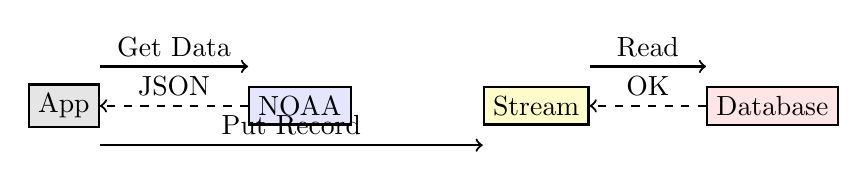
\begin{tikzpicture}[node distance=3cm, auto, thick]
    % Nodes
    \node (App) [rectangle, draw, fill=gray!20] {App};
    \node (API) [rectangle, draw, fill=blue!10, right of=App] {NOAA};
    \node (Stream) [rectangle, draw, fill=yellow!20, right of=API] {Stream};
    \node (DB) [rectangle, draw, fill=red!10, right of=Stream] {Database};

    \draw [->] ([yshift=0.5cm]App.east) -- node[above] {Get Data} ([yshift=0.5cm]API.west);
    \draw [->, dashed] ([yshift=0.0cm]API.west) -- node[above] {JSON} ([yshift=0.0cm]App.east);
    
    \draw [->] ([yshift=-0.5cm]App.east) -- node[above] {Put Record} ([yshift=-0.5cm]Stream.west);
    
    \draw [->] ([yshift=0.5cm]Stream.east) -- node[above] {Read} ([yshift=0.5cm]DB.west);
    \draw [->, dashed] ([yshift=0.0cm]DB.west) -- node[above] {OK} ([yshift=0.0cm]Stream.east);
    
\end{tikzpicture}
\caption{Process Flow}
\end{figure}

\newpage

\section{Building the Producer}

The Producer is the start of our pipeline. It's a Python script (`producer.py`) that acts like a specialized web browser. It visits the NOAA website (via API), gets the data, and passes it on.

\subsection{Handling the NOAA API}
The API is strict—it only allows 5 requests per second. If we go faster, it blocks us. so we added a `time.sleep(0.2)` command.

Here is the core loop that fetches the stations:

\begin{lstlisting}[language=Python, caption=Fetching Stations Safely]
def get_maryland_stations(self):
    url = f"{self.base_url}/stations"
    params = {
        'locationid': 'FIPS:24',  # Maryland
        'datasetid': 'GHCND',
        'limit': 1000
    }
    
    while True:
        # Ask the API for data
        response = requests.get(url, headers=self.headers, params=params)
        data = response.json()
        
        # Add to our list
        stations.extend(data['results'])
        
        # IMPORTANT: Wait a bit to be polite to the API
        time.sleep(0.2) 
        
        # If no more data, stop
        if len(data['results']) < 1000:
            break
            
    return stations
\end{lstlisting}

\subsection{Sending to Kinesis}
Once we have the data, we send it to AWS. We use the `boto3` library, which is the official AWS tool for Python.

\begin{lstlisting}[language=Python, caption=Sending Data]
def send_to_kinesis(self, record):
    # Convert our dictionary to a text string (JSON)
    payload = json.dumps(record)
    
    # Send it!
    self.kinesis_client.put_record(
        StreamName='weather-data-stream',
        Data=payload,
        PartitionKey=record['station_id']
    )
\end{lstlisting}

Using `PartitionKey` is a cool trick. By setting it to `station_id`, we tell AWS: "Keep all records for Station X together." This ensures that if we read the data later, Station X's Monday report comes before its Tuesday report.

\newpage

\section{Building the Consumer}

The Consumer (`consumer.py`) is where the real work happens. It reads the raw data and organizes it.

\subsection{The Challenge: Numbers in Computers}
We hit an interesting bug during this project. Python uses "Floats" for decimal numbers (like `12.5`). DynamoDB uses "Decimals". They sound the same, but to a computer, they are very different. If you try to send a Python Float to DynamoDB, it gives an error.

We wrote a helper function to fix this:

\begin{lstlisting}[language=Python, caption=Fixing the Number Format]
from decimal import Decimal

def convert_floats(obj):
    # If it's a list, fix every item in the list
    if isinstance(obj, list):
        return [convert_floats(item) for item in obj]
    
    # If it's a dictionary, fix every value
    elif isinstance(obj, dict):
        return {k: convert_floats(v) for k, v in obj.items()}
        
    # If it's a float, turn it into a Decimal
    elif isinstance(obj, float):
        return Decimal(str(obj))
        
    # Otherwise, leave it alone
    return obj
\end{lstlisting}

\subsection{Saving to DynamoDB}
We split the data into two tables. This keeps our data clean.

\begin{lstlisting}[language=Python, caption=Saving Precipitation Data]
def store_precipitation(self, station_id, date, precip, snow):
    item = {
        'station_id': station_id,  # Main ID
        'timestamp': date,         # Sort by date
        'type': 'precipitation'
    }
    
    # Only add snow if we actually have data for it
    if snow is not None:
        item['snow_mm'] = Decimal(str(snow))
    
    if precip is not None:
        item['precip_mm'] = Decimal(str(precip))
        
    self.table.put_item(Item=item)
\end{lstlisting}

\newpage

\section{Monitoring the System}

How do we know if it's working? We wrote a monitor script (`monitor_pipeline.py`) that asks AWS for health metrics.

The most important number to watch is **Iterator Age**.
\begin{itemize}
    \item **Iterator Age = 0**: The Consumer is caught up. It's reading data the moment it arrives.
    \item **Iterator Age > 0**: The Consumer is falling behind. The data is "aging" in the stream before being read.
\end{itemize}

Here is how we check it:

\begin{lstlisting}[language=Python, caption=Health Check]
def check_health(self):
    # Ask CloudWatch for the stats
    stats = self.cloudwatch.get_metric_statistics(
        Namespace='AWS/Kinesis',
        MetricName='GetRecords.IteratorAgeMilliseconds',
        Dimensions=[{'Name': 'StreamName', 'Value': 'weather-stream'}],
        Statistics=['Maximum']
    )
    
    age_seconds = stats['Datapoints'][0]['Maximum'] / 1000
    
    print(f"Current Lag: {age_seconds} seconds")
    
    if age_seconds > 60:
        print("WARNING: We are falling behind!")
    else:
        print("System is healthy.")
\end{lstlisting}

\section{Cost Analysis}

One concern with cloud projects is cost. "Will this accidentally cost me \$1000?"
For this project, the answer is **no**. It is very cheap.

Here is the breakdown for running this for a full month:

\begin{table}[H]
\centering
\begin{tabular}{llc}
\toprule
\textbf{Service} & \textbf{Usage} & \textbf{Est. Cost} \\
\midrule
Kinesis Stream & 730 hours (1 Shard) & \$10.95 \\
Data Put Requests & 1 Million records & \$0.01 \\
DynamoDB Writes & ~25 Units/sec & \$12.35 \\
DynamoDB Reads & ~5 Units/sec & \$0.95 \\
\midrule
\textbf{Total Monthly} & & \textbf{\$24.26} \\
\bottomrule
\end{tabular}
\caption{Estimated Monthly Bill}
\end{table}

This is much cheaper than renting a dedicated server (EC2 instance) and a SQL database, which could easily cost over \$50/month.

\section{How to Run It}

If you want to run this project yourself, follow these steps.

\subsection{1. Setup}
Make sure you have Python installed and your AWS keys set up.
\begin{verbatim}
pip install boto3 requests python-dotenv
\end{verbatim}

\subsection{2. Configuration}
Create a file named `.env` and add your keys:
\begin{verbatim}
NOAA_TOKEN=your_token_here
KINESIS_STREAM_NAME=weather-data-stream
\end{verbatim}

\subsection{3. Run the Producer}
Start the script that fetches data. It will print out what it's doing.
\begin{verbatim}
python producer.py
\end{verbatim}
\textit{Output: Found 420 stations... Fetching data... Sent 50 records...}

\subsection{4. Run the Consumer}
In a new terminal window, start the consumer.
\begin{verbatim}
python consumer.py
\end{verbatim}
\textit{Output: Connected to stream... Processed 50 records... Saved to DynamoDB...}

\section{Conclusion}

This project showed how easy it is to build a professional-grade data pipeline using AWS tools. By using Kinesis and DynamoDB, we built a system that is:
\begin{itemize}
    \item **Resilient**: If the database slows down, Kinesis holds the data.
    \item **Scalable**: If we want to track the whole USA instead of just Maryland, we just add more Kinesis "Shards".
    \item **Simple**: The Python code is clean and easy to read.
\end{itemize}

This architecture is exactly what big companies use, just on a smaller scale. It's a great foundation for any real-time data project.

\end{document}
